\section{Materiais e Métodos}
\subsection{Materiais}
Para captar e realizar a leitura do ruído eletromagnético foram utilizados uma antena para a captação
e um microcontrolador para a aquisição do valor do ruído captado.
\subsubsection{Arduino UNO}
O Arduino Uno (Fig 1) é uma placa de microcontrolador baseado no ATmega328 (datasheet). Possui 14 pinos de entrada/saída digital (dos quais 6 podem ser usados como saídas PWM), 6 entradas analógicas, um cristal oscilador de 16MHz, uma conexão USB e uma entrada de alimentação uma conexão ICSP.

O microcontrolador foi responsável pela leitura do ruído eletromagnético em uma de suas portas analógicas. O ruído foi então convertido para um valor numérico através do conversor analógico-digital (ADC) presente no Arduino.

\begin{figure}[H]
	\label{fig1}
	\begin{centering}
		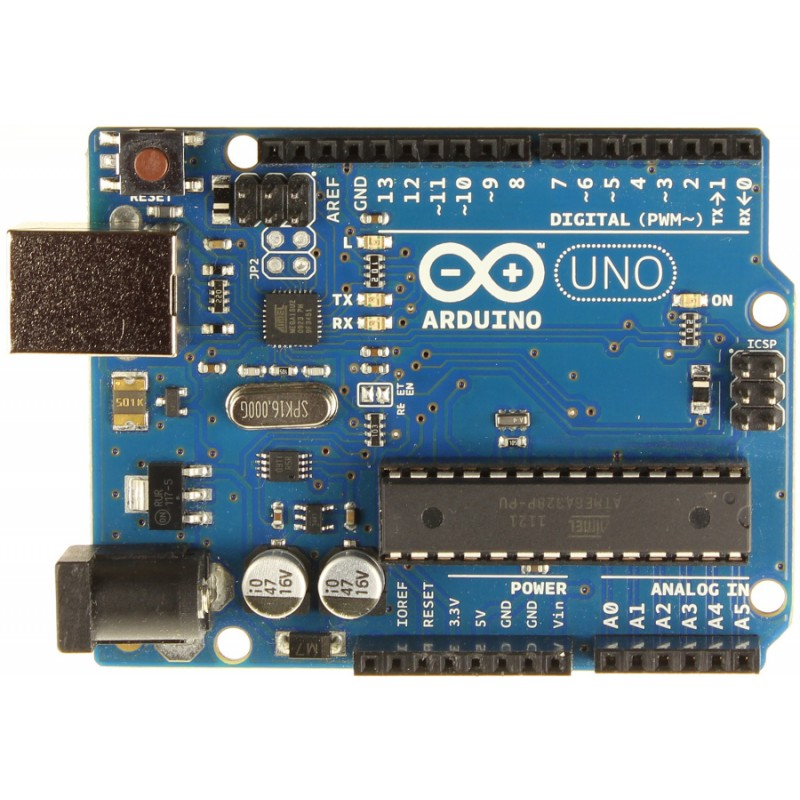
\includegraphics[width = 400pt]{img/arduino.jpg}
		\caption{Arduino UNO}
	\end{centering}	
		
\end{figure}

\subsubsection{Antena}

Foi utilizado um fio de estanho na porta do microcontrolador como aparato para a captação de interferência eletromagnética. A configuração escolhida da antena foi de monopolo de quarto de onda \cite{Balanis2005}.
A frequência captada pela antena é prevista pela equação abaixo:

\begin{equation}
   f = \frac{c}{\frac{L}{4}}
  \end{equation}
sendo $f$ a frequência em Herz, $c$ a velocidade da luz e $L$ o comprimento da antena. Para uma antena de 8 centímetros, a frequência
captada pela antena é de 15MHz.
 \begin{figure}[H]
 	\label{fig2}
 	\begin{centering}
 		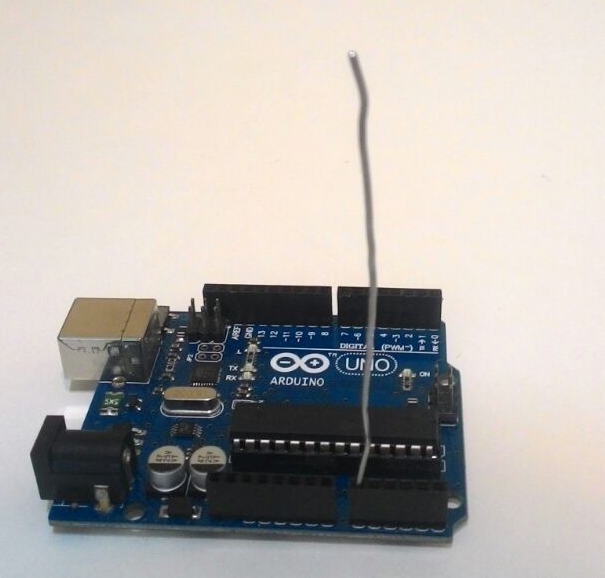
\includegraphics[width = 200pt]{img/arduino2.png}
 		\caption{Arduino UNO com a antena monopolo}
 	\end{centering}	
 		
 \end{figure}

\subsection{Métodos}